
\begin{center}
\begin{figure}[H]
    \centering
    \begin{subfigure}[b]{0.48\linewidth}
        \centering
        
\includegraphics[height=2cm, keepaspectratio]{images/UFR.png}
    \end{subfigure}
    \hfill
    \begin{subfigure}[b]{0.48\linewidth}
        \centering
        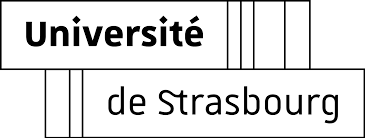
\includegraphics[height=2cm, keepaspectratio]{images/images.png}
    \end{subfigure}
\end{figure}

    \vfill

    {
	\large
	\textsc{
	       Master 1 Image et 3D
	}
    }

    \bigskip\bigskip
    \bigskip\bigskip

    {\huge Travail d'étude et de recherche}

    \bigskip\bigskip

    % Identité de l'auteur
    
    {\large Axel \textsc{FRANZ}}
    
    \vfill

    % Titre du TER : mettez un titre utile
    {
	\huge
	\textsc{
	    Procedural water rendering using tile animation
	}
    }

    \vfill
    \vfill

    \vfill

    {\large Projet encadré par}

    \medskip

    {\large Romain \textsc{FOURNIER}}
    \\
    {\large Basile \textsc{SAUVAGE}}

    \bigskip

    \bigskip

\end{center}


\newpage